%!TEX root = ../../thesis.tex

\section{Feature Encoding}
\label{methodology:feature_encoding}

The feature encoding section of FlatCityBuf is responsible for the binary representation of 3D city objects and their associated data. This component preserves the semantic richness of the CityJSON model while leveraging FlatBuffers' efficient binary serialisation. The full schema definition for feature encoding can be found in \autoref{appendix:flatcitybuf_schema:feature}.

\subsection{CityJSONFeature and CityObject Structure}
\label{methodology:feature_encoding:cityfeature_cityobject_structure}

FlatCityBuf implements the core structure of \ac{cjseq} using the following FlatBuffers tables:

\begin{itemize}
  \item \textbf{CityFeature} - \textit{table (root object)} - The top-level container for city objects:
    The CityFeature properties are detailed in \autoref{tab:cityfeature_properties}.

    \begin{table}[h]
      \centering
      \caption{CityFeature properties in the FlatCityBuf feature encoding}
      \label{tab:cityfeature_properties}
      \small
      \begin{tabularx}{\textwidth}{@{}llX@{}}
        \toprule
        \textbf{Property} & \textbf{Data Type} & \textbf{Description} \\
        \midrule
        id & string (key, required) & Required string identifier, marked as a key field for fast lookup \\
        objects & Array of CityObject tables & Collection of individual 3D features \\
        vertices & Array of Vertex structs & Quantized X,Y,Z coordinates (int32) \\
        appearance & Appearance table & Optional visual styling information \\
        \bottomrule
      \end{tabularx}
    \end{table}

  \item \textbf{CityObject} - \textit{table} - Individual 3D city objects with properties detailed in \autoref{tab:cityobject_properties}

    \begin{table}[h]
      \centering
      \caption{CityObject properties in the FlatCityBuf feature encoding}
      \label{tab:cityobject_properties}
      \small
      \begin{tabularx}{\textwidth}{@{}llX@{}}
        \toprule
        \textbf{Property} & \textbf{Data Type} & \textbf{Description} \\
        \midrule
        type & CityObjectType enum & Object classification (Building, Bridge, etc.) following CityJSON types \\
        id & string (key, required) & Required string identifier, marked as a key field \\
        geographical\_extent & GeographicalExtent struct & 3D bounding box of the object \\
        geometry & Array of Geometry tables & Shape information \\
        attributes & ubyte array & Binary blob containing attribute values (interpretable via columns schema) \\
        columns & Array of Column tables & Schema defining attribute types and names \\
        children & Array of string & IDs referencing child objects \\
        children\_roles & Array of string & Descriptions of relationship roles \\
        parents & Array of string & IDs referencing parent objects \\
        extension\_type & string & Optional type for extended objects (e.g., "+NoiseBuilding") \\
        \bottomrule
      \end{tabularx}
    \end{table}
\end{itemize}

This structure maintains CityJSON's hierarchical organisation while taking advantage of FlatBuffers' binary encoding and zero-copy access capabilities, with the exception of attributes which are self-encoded as binary blobs.

\subsection{Geometry Encoding}
\label{methodology:feature_encoding:geometry_encoding}

Geometry in FlatCityBuf follows CityJSON's boundary representation (B-rep) model with flattened arrays for FlatBuffers encoding:

\begin{itemize}
  \item \textbf{Geometry} - \textit{table} - Container for geometric representation with properties detailed in \autoref{tab:geometry_properties}

    \begin{table}[h]
      \centering
      \caption{Geometry properties in the FlatCityBuf feature encoding}
      \label{tab:geometry_properties}
      \small
      \begin{tabularx}{\textwidth}{@{}llX@{}}
        \toprule
        \textbf{Property} & \textbf{Data Type} & \textbf{Description} \\
        \midrule
        type & GeometryType enum & Geometric dimension type (0D-Point, 1D-LineString, etc.) \\
        lod & float & Level of Detail value \\
        boundaries & Array of uint32 & Indices referencing vertices \\
        strings & Array of uint32 & Counts defining vertex groups \\
        surfaces & Array of uint32 & Counts defining string groups \\
        shells & Array of uint32 & Counts defining surface groups \\
        solids & Array of uint32 & Counts defining shell groups \\
        semantics\_boundaries & Array of uint32 & Parallel arrays to boundaries for semantic classification \\
        semantics\_values & Array of SemanticObject tables & Semantic information for surfaces \\
        \bottomrule
      \end{tabularx}
    \end{table}

  \item \textbf{SemanticObject} - \textit{table} - Semantic classification of geometry parts with properties detailed in \autoref{tab:semanticobject_properties}

    \begin{table}[h]
      \centering
      \caption{SemanticObject properties in the FlatCityBuf feature encoding}
      \label{tab:semanticobject_properties}
      \small
      \begin{tabularx}{\textwidth}{@{}llX@{}}
        \toprule
        \textbf{Property} & \textbf{Data Type} & \textbf{Description} \\
        \midrule
        type & SemanticSurfaceType enum & Surface classification (WallSurface, RoofSurface, etc.) \\
        extension\_type & string & Optional extended semantic type name \\
        attributes & ubyte array & Binary blob containing semantic-specific attributes \\
        columns & Array of Column tables & Schema defining attribute types and names \\
        parent & uint32 & Index to parent semantic object \\
        children & Array of uint32 & Indices to child semantic objects \\
        \bottomrule
      \end{tabularx}
    \end{table}

  \item \textbf{GeometryInstance} - \textit{table} - Reference to template geometry with properties detailed in \autoref{tab:geometryinstance_properties}

    \begin{table}[h]
      \centering
      \caption{GeometryInstance properties in the FlatCityBuf feature encoding}
      \label{tab:geometryinstance_properties}
      \small
      \begin{tabularx}{\textwidth}{@{}llX@{}}
        \toprule
        \textbf{Property} & \textbf{Data Type} & \textbf{Description} \\
        \midrule
        transformation & TransformationMatrix struct & 4×4 transformation matrix \\
        template & uint32 & Index referencing a template in the header section \\
        boundaries & Array of uint32 & Single-element array containing reference point index \\
        \bottomrule
      \end{tabularx}
    \end{table}

  \item \textbf{Vertex} - \textit{struct} - Quantized 3D coordinates with properties detailed in \autoref{tab:vertex_properties}

    \begin{table}[h]
      \centering
      \caption{Vertex properties in the FlatCityBuf feature encoding}
      \label{tab:vertex_properties}
      \small
      \begin{tabularx}{\textwidth}{@{}llX@{}}
        \toprule
        \textbf{Property} & \textbf{Data Type} & \textbf{Description} \\
        \midrule
        x & int32 & X coordinate, converted using header transform \\
        y & int32 & Y coordinate, converted using header transform \\
        z & int32 & Z coordinate, converted using header transform \\
        \bottomrule
      \end{tabularx}
    \end{table}
\end{itemize}

\subsubsection{Hierarchical Boundaries as Flattened Arrays}
\label{methodology:feature_encoding:geometry_encoding:flattened_arrays}

A key challenge in adapting CityJSON's recursive boundary representation to FlatBuffers is that FlatBuffers does not support nested arrays. FlatCityBuf addresses this by implementing a dimensional hierarchy encoded as parallel flattened arrays:

The encoding strategy follows a dimensional hierarchy from lowest to highest dimension:

\begin{enumerate}
  \item \textbf{boundaries}: A single flattened array of integer vertex indices
  \item \textbf{strings}: Array where each value indicates the number of vertices in each ring/boundary
  \item \textbf{surfaces}: Array where each value indicates the number of strings/rings in each surface
  \item \textbf{shells}: Array where each value indicates the number of surfaces in each shell
  \item \textbf{solids}: Array where each value indicates the number of shells in each solid
\end{enumerate}

\begin{figure}[ht]
  \centering
  \begin{minipage}{0.45\textwidth}
    \centering
    
\includegraphics[width=\textwidth]{./figs/methodology/triangle.png}
    \caption{Example of a triangle encoded as a hierarchical boundary.}
    \label{fig:triangle_encoding}
  \end{minipage}
  \hfill
  \begin{minipage}{0.45\textwidth}
    \centering
    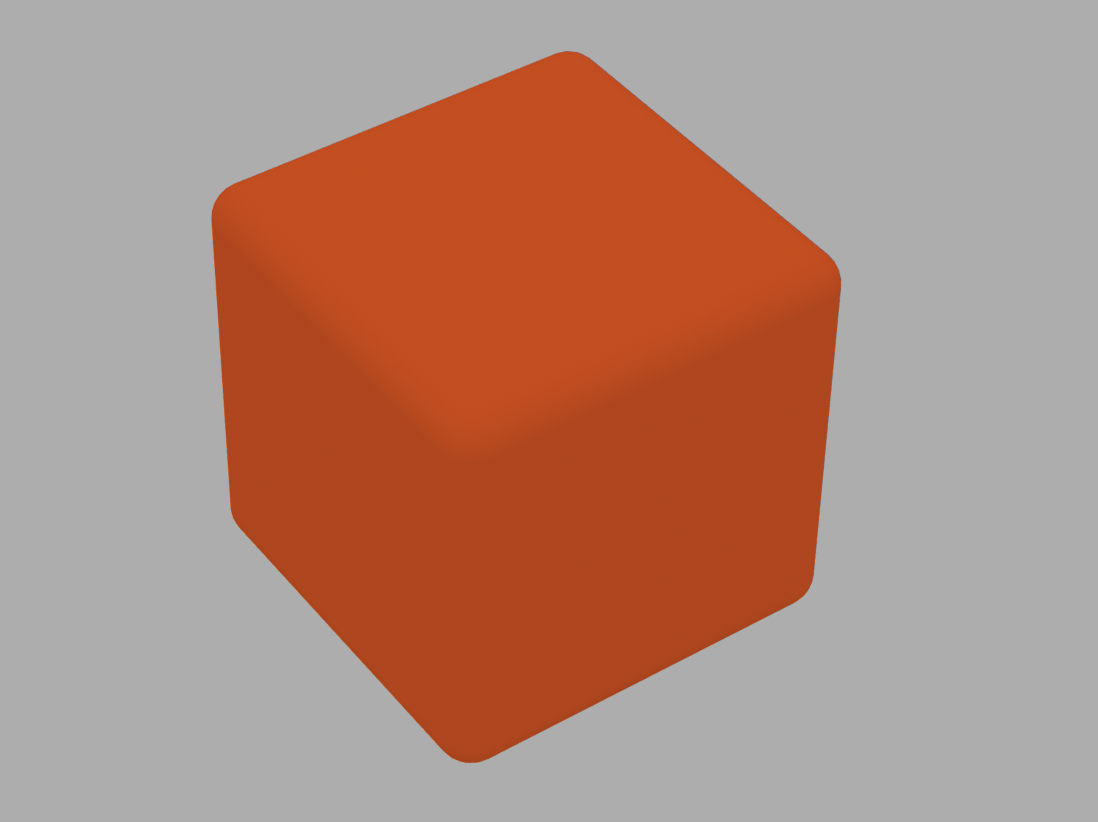
\includegraphics[width=\textwidth]{./figs/methodology/cube.png}
    \caption{Example of a cube encoded as a hierarchical boundary.}
    \label{fig:cube_encoding}
  \end{minipage}
\end{figure}

For example, a simple triangle would be encoded as:
\begin{lstlisting}[caption={Hierarchical boundary encoding for a simple triangle}, label={lst:triangle_encoding}, basicstyle=\small\ttfamily]
boundaries: [0, 1, 2]       // Indices of three vertices
strings: [3]                // Single string with 3 vertices
surfaces: [1]               // Single surface containing 1 string
\end{lstlisting}

A more complex structure such as a cube (a solid with 6 quadrilateral faces) would be encoded as:

\begin{lstlisting}[caption={Hierarchical boundary encoding for a cube structure}, label={lst:cube_encoding}, basicstyle=\small\ttfamily, breaklines=true]
boundaries: [0, 1, 2, 3, 0, 3, 7, 4, 1, 5, 6, 2, 4, 7, 6, 5, 0, 4, 5, 1, 2, 6, 7, 3]
strings: [4, 4, 4, 4, 4, 4]    // 6 strings with 4 vertices each
surfaces: [1, 1, 1, 1, 1, 1]   // 6 surfaces with 1 string each
shells: [6]                    // 1 shell with 6 surfaces
solids: [1]                    // 1 solid with 1 shell
\end{lstlisting}

\subsubsection{Semantic Surface Encoding}
\label{methodology:feature_encoding:geometry_encoding:semantics}

Semantic surface information is encoded using a similar approach:

\begin{itemize}
  \item \textbf{semantics\_values}: Array of \textit{SemanticObject} tables containing type classifications, attributes, and hierarchical relationships
  \item \textbf{semantics\_boundaries}: Array of indices that reference entries in \textit{semantics\_values}, with a parallel structure to the geometry boundaries
\end{itemize}

This parallel structure allows each geometric component to have associated semantic information without requiring deeply nested structures. For example, in a building model where each face has a semantic classification (wall, roof, etc.), the \textit{semantics\_boundaries} array would have the same structure as the \textit{boundaries} array, with each surface having a corresponding semantic value.

Through this flattened array approach, FlatCityBuf preserves the rich hierarchical structure of CityJSON geometries while conforming to FlatBuffers' efficiency-oriented constraints on data organisation.

\subsubsection{Geometry Template Encoding}
\label{methodology:feature_encoding:geometry_encoding:templates}

FlatCityBuf implements CityJSON's template mechanism for efficient representation of repeated geometry patterns, a common requirement in urban environments where many buildings, street furniture items, vegetation, or other objects share identical geometric structures. The template approach separates the geometry definition from its instantiation:

\begin{itemize}
  \item \textbf{Template Definition}: Templates are defined once in the header section as full Geometry objects with characteristics detailed in \autoref{tab:template_definition}

    \begin{table}[h]
      \centering
      \caption{Template Definition characteristics in FlatCityBuf geometry templates}
      \label{tab:template_definition}
      \small
      \begin{tabularx}{\textwidth}{@{}lX@{}}
        \toprule
        \textbf{Characteristic} & \textbf{Description} \\
        \midrule
        Geometry format & Templates use the same Geometry table format described previously for standard geometries \\
        Vertex precision & Template vertices are stored with double-precision coordinates (\texttt{DoubleVertex}) to maintain accuracy in the local coordinate system \\
        Vertex storage & All template vertices for all templates are stored in a single flat array (\texttt{templates\_vertices}) \\
        Index referencing & Indices within template boundaries reference positions in this dedicated template vertex array \\
        \bottomrule
      \end{tabularx}
    \end{table}

  \item \textbf{Template Instantiation}: CityObjects reference templates through GeometryInstance tables with properties detailed in \autoref{tab:template_instantiation}

    \begin{table}[h]
      \centering
      \caption{Template Instantiation properties in FlatCityBuf geometry templates}
      \label{tab:template_instantiation}
      \small
      \begin{tabularx}{\textwidth}{@{}llX@{}}
        \toprule
        \textbf{Property} & \textbf{Data Type} & \textbf{Description} \\
        \midrule
        template & uint & A single unsigned integer index referencing a specific template in the header \\
        boundaries & Array of uint & Contains exactly one index referencing a vertex in the feature's vertex array, which serves as the reference point for placement \\
        transformation & TransformationMatrix & A 4×4 transformation matrix (rotation, translation, scaling) that positions the template relative to the reference point \\
        \bottomrule
      \end{tabularx}
    \end{table}
\end{itemize}

FlatCityBuf preserves CityJSON's template mechanism, which provides significant storage efficiency by storing repeated geometries once and referencing them with transformation parameters.

\subsection{Materials and Textures}
\label{methodology:feature_encoding:materials_textures}

FlatCityBuf supports CityJSON's appearance model through the following structures:

\begin{itemize}
  \item \textbf{Appearance} - \textit{table} - Container for visual styling information with properties detailed in \autoref{tab:appearance_feature_properties}

    \begin{table}[h]
      \centering
      \caption{Appearance properties in FlatCityBuf feature encoding}
      \label{tab:appearance_feature_properties}
      \small
      \begin{tabularx}{\textwidth}{@{}llX@{}}
        \toprule
        \textbf{Property} & \textbf{Data Type} & \textbf{Description} \\
        \midrule
        materials & Array of Material tables & Surface visual properties definitions \\
        textures & Array of Texture tables & Image mapping information \\
        vertices\_texture & Array of Vec2 structs & UV coordinates for texture mapping \\
        material\_mapping & Array of MaterialMapping tables & Links materials to surfaces \\
        texture\_mapping & Array of TextureMapping tables & Links textures to surfaces \\
        default\_theme\_material & string & Default material theme identifier \\
        default\_theme\_texture & string & Default texture theme identifier \\
        \bottomrule
      \end{tabularx}
    \end{table}

  \item \textbf{Material} - \textit{table} - Surface visual properties with properties detailed in \autoref{tab:material_feature_properties}

    \begin{table}[h]
      \centering
      \caption{Material properties in FlatCityBuf feature encoding}
      \label{tab:material_feature_properties}
      \small
      \begin{tabularx}{\textwidth}{@{}llX@{}}
        \toprule
        \textbf{Property} & \textbf{Data Type} & \textbf{Description} \\
        \midrule
        name & string (required) & Unique material identifier \\
        ambient\_intensity & double & Value from 0.0 to 1.0 \\
        diffuse\_color & Array of double & RGB values from 0.0 to 1.0 \\
        emissive\_color & Array of double & RGB values from 0.0 to 1.0 \\
        specular\_color & Array of double & RGB values from 0.0 to 1.0 \\
        shininess & double & Value from 0.0 to 128.0 \\
        transparency & double & Value from 0.0 to 1.0 \\
        is\_smooth & boolean & Flag for smooth shading \\
        \bottomrule
      \end{tabularx}
    \end{table}

  \item \textbf{Texture} - \textit{table} - Image mapping information with properties detailed in \autoref{tab:texture_feature_properties}

    \begin{table}[h]
      \centering
      \caption{Texture properties in FlatCityBuf feature encoding}
      \label{tab:texture_feature_properties}
      \small
      \begin{tabularx}{\textwidth}{@{}llX@{}}
        \toprule
        \textbf{Property} & \textbf{Data Type} & \textbf{Description} \\
        \midrule
        type & TextureFormat enum & Format type (PNG, JPG) \\
        image & string (required) & Image file name or URL \\
        wrap\_mode & WrapMode enum & Wrapping option (None, Wrap, Mirror, Clamp, Border) \\
        texture\_type & TextureType enum & Type classification (Unknown, Specific, Typical) \\
        border\_color & Array of double & RGBA values from 0.0 to 1.0 \\
        \bottomrule
      \end{tabularx}
    \end{table}

  \item \textbf{MaterialMapping} - \textit{table} - Links materials to surfaces with properties detailed in \autoref{tab:materialmapping_properties}

    \begin{table}[h]
      \centering
      \caption{MaterialMapping properties in FlatCityBuf feature encoding}
      \label{tab:materialmapping_properties}
      \small
      \begin{tabularx}{\textwidth}{@{}llX@{}}
        \toprule
        \textbf{Property} & \textbf{Data Type} & \textbf{Description} \\
        \midrule
        theme & string & Theme identifier (e.g., "summer", "winter") \\
        values & Array of uint32 & Indices to surfaces or boundaries \\
        material & uint32 & Index to the referenced material \\
        \bottomrule
      \end{tabularx}
    \end{table}

  \item \textbf{TextureMapping} - \textit{table} - Links textures to surfaces with properties detailed in \autoref{tab:texturemapping_properties}

    \begin{table}[h]
      \centering
      \caption{TextureMapping properties in FlatCityBuf feature encoding}
      \label{tab:texturemapping_properties}
      \small
      \begin{tabularx}{\textwidth}{@{}llX@{}}
        \toprule
        \textbf{Property} & \textbf{Data Type} & \textbf{Description} \\
        \midrule
        theme & string & Theme identifier (e.g., "summer", "winter") \\
        values & Array of uint32 & Indices to surfaces or boundaries \\
        texture & uint32 & Index to the referenced texture \\
        uv\_indexes & Array of uint32 & Indices to UV coordinates \\
        \bottomrule
      \end{tabularx}
    \end{table}
\end{itemize}

This implementation prioritizes efficient storage by referencing external texture files rather than embedding image data directly, enabling selective loading based on application requirements while maintaining full compatibility with CityJSON's appearance model.

\subsubsection{Texture Storage Design Rationale}
\label{methodology:feature_encoding:textures:rationale}

FlatCityBuf stores texture references rather than embedding texture data directly for several strategic reasons:

\begin{itemize}
  \item \textbf{Performance Priority}: Enables rapid loading of geometric and semantic data without the overhead of large texture files when not required.

  \item \textbf{On-demand Loading}: Supports selective texture loading based on application needs, beneficial for analysis-focused use cases.

  \item \textbf{Size Management}: Maintains reasonable file sizes for large-scale datasets.

  \item \textbf{Web Efficiency}: Individual texture files can be cached by browsers or \ac{cdn}s, significantly improving performance for repeated access in web applications.
\end{itemize}

This approach follows established patterns in formats like glTF, OBJ, and I3S, prioritizing operational efficiency over self-contained packaging for city-scale datasets.

\subsection{Attribute Encoding}
\label{methodology:feature_encoding:attribute_encoding}

Attributes in FlatCityBuf are encoded as binary data with a schema defined through \textit{Column} tables, which were detailed previously in \autoref{methodology:header:schema_indexing}. Rather than repeating column structure information, this section focuses on the binary encoding strategy:

\begin{itemize}
  \item \textbf{Attribute Binary Encoding} - Efficient type-specific serialisation:
    \begin{itemize}
      \item \textit{Numeric types} - Native binary representation (little-endian)
      \item \textit{String} - Length-prefixed UTF-8 encoding
      \item \textit{Boolean} - Single byte (0 = false, 1 = true)
      \item \textit{Date/DateTime} - Standardized binary format
      \item \textit{Byte array} - Length-prefixed binary data
      \item \textit{Nested JSON} - Length-prefixed JSON string encoding of complex nested structures
      \item \textit{Null} - Not encoded to save space (null attributes are omitted from the binary representation)
    \end{itemize}
\end{itemize}

FlatCityBuf encodes attributes as type-specific binary values with a corresponding schema definition. Each attribute is stored as a key-value pair where the key is the column index and the value is the binary representation of the attribute. This approach balances flexibility with reasonable performance while maintaining compatibility with the original CityJSON semantic model. The figure below illustrates how different attribute types are encoded in the binary format.

\begin{figure}[htbp]
  \centering
  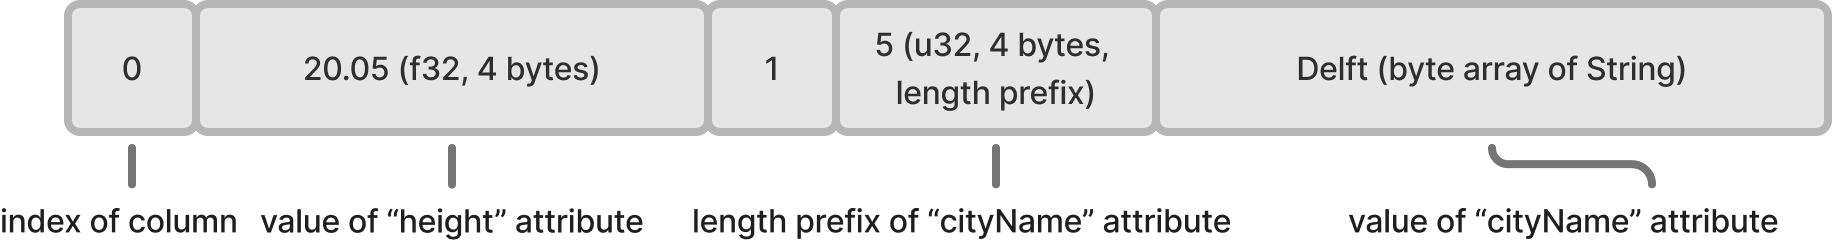
\includegraphics[width=0.8\textwidth]{figs/methodology/attribute_structure.png}
  \caption{Example of attribute encoding in FlatCityBuf}
  \label{methodology:feature_encoding:attribute_encoding:figure}
\end{figure}

\subsection{Extension Mechanism}
\label{methodology:feature_encoding:extension_mechanism}

FlatCityBuf provides comprehensive support for CityJSON's Extension mechanism, which was previously detailed in \autoref{methodology:header:extensions}. While the Extension structures are defined in the header, their implementation within actual city features requires specific encoding strategies that balance extensibility with performance.

\subsubsection{Encoding of Extended City Objects}
\label{methodology:feature_encoding:extension_mechanism:city_objects}

Extended city object types (those prefixed with "+") are encoded using a two-part strategy:

\begin{itemize}
  \item A standard enum value \texttt{ExtensionObject} is used for the \texttt{type} field to distinguish whether the extended object or core object
  \item The actual extension type name (e.g., "+NoiseCityFurnitureSegment") is stored in the \texttt{extension\_type} string field (This will be null for core objects)
\end{itemize}

\subsubsection{Encoding of Extended Semantic Surfaces}
\label{methodology:feature_encoding:extension_mechanism:semantic_surfaces}

Similarly, extended semantic surface types follow the same pattern:

\begin{itemize}
  \item The \texttt{type} field uses the enum value \texttt{ExtraSemanticSurface}
  \item The specific type (e.g., "+ThermalSurface") is stored in the \texttt{extension\_type} field (This will be null for core objects)
\end{itemize}

\subsubsection{Extension Attribute Encoding}
\label{methodology:feature_encoding:extension_mechanism:attributes}

Extension-specific attributes are encoded using the same binary serialisation mechanism as core attributes:

\begin{itemize}
  \item Extension attributes are included in the same binary representation as standard attributes
  \item The schema for these attributes is stored alongside the \texttt{columns} of the \texttt{Header} table (See \autoref{methodology:header:schema_indexing})
\end{itemize}

During decoding:
\begin{itemize}
  \item The same decoding logic is applied as for core attributes
  \item If needed, the application can identify extension attributes by checking if the column name begins with "+"
\end{itemize}

\subsubsection{Adding New Properties at the Root of a Document}
\label{methodology:feature_encoding:extension_mechanism:adding_new_properties_at_the_root_of_a_document}

Adding new properties at the root level follows the same principle as adding extension attributes to existing City Objects. Since root-level extensions are also arbitrary structured JSON objects, fields starting with "+" are treated as extension attributes. The attribute encoding mechanism does not distinguish whether attribute keys start with "+" or not, so no special treatment is required.

However, since each City Object can already have extended attributes, this approach is rarely needed in practice. Consequently, we have not yet implemented this functionality.

Unlike CityJSON, which references external schema files for extensions, FlatCityBuf's self-contained approach ensures that all extension information is available within a single file. This approach maintains the cloud-optimised philosophy of minimising external dependencies while preserving full compatibility with the rich extension capabilities of CityJSON.
